\chapter{Wyniki eksperymentów}
\label{chap:wyniki}

W tym rozdziale przedstawiam wyniki eksperymentów przeprowadzonych
zgodnie z metodyką opisaną w rozdziale~\ref{chap:eksperymenty}.
Analizuję jakość końcowych strategii, wpływ reprezentacji stanu
i funkcji nagrody, przebieg procesu uczenia oraz zachowanie modeli po
zwiększeniu budżetu treningowego.

Podstawę głównej analizy stanowi osiem konfiguracji powstałych
z połączenia dwóch algorytmów, dwóch reprezentacji stanu oraz dwóch
funkcji nagrody. Każdą konfigurację wytrenowałem pięciokrotnie
z wykorzystaniem tego samego zestawu pięciu seedów treningowych.
Końcową ocenę każdego modelu przeprowadziłem na wspólnym harmonogramie
100\,000 rozdań, który nie był wykorzystywany podczas treningu,
walidacji ani wyboru konfiguracji.

Jako podstawową miarę jakości strategii wykorzystuję średni zysk netto
na rozdanie, wyrażony w jednostkach zakładu Ante. Wartości bliższe zeru
oznaczają mniejszą średnią stratę gracza, natomiast wartość dodatnia
oznaczałaby strategię osiągającą dodatni średni wynik w badanej próbie.

\section{Wyniki końcowej ewaluacji}
\label{sec:wyniki-koncowej-ewaluacji}

W pierwszej kolejności porównałem końcowe wyniki wszystkich ośmiu
podstawowych konfiguracji po 50\,000 epizodów treningowych.
Dla każdej konfiguracji obliczyłem średnią wartość EV z pięciu
niezależnych przebiegów treningowych oraz odchylenie standardowe między
seedami. Wyniki przedstawiam w tabeli~\ref{tab:final-ev-50k}.

\begin{table}[htbp]
    \centering
    \caption{Wyniki końcowej ewaluacji modeli po 50\,000 epizodów treningowych}
    \label{tab:final-ev-50k}
    \begin{tabular}{lllrr}
        \toprule
        Algorytm & Reprezentacja & Nagroda & Średnie EV & SD seedów \\
        \midrule
        DQN & RAW & zysk netto
            & -0{,}6450 & 0{,}0184 \\
        DQN & RAW & skalowana
            & -0{,}5681 & 0{,}0401 \\
        DQN & FEATURES & zysk netto
            & -0{,}4076 & 0{,}0080 \\
        DQN & FEATURES & skalowana
            & -0{,}4165 & 0{,}0169 \\
        \midrule
        REINFORCE & RAW & zysk netto
            & -0{,}3785 & 0{,}0074 \\
        REINFORCE & RAW & skalowana
            & -0{,}3804 & 0{,}0014 \\
        REINFORCE & FEATURES & zysk netto
            & -0{,}3823 & 0{,}0014 \\
        REINFORCE & FEATURES & skalowana
            & -0{,}3211 & 0{,}0657 \\
        \bottomrule
    \end{tabular}
\end{table}

Najwyższe średnie EV spośród wariantów DQN uzyskała konfiguracja
FEATURES z funkcją nagrody opartą na zysku netto. Jej średni wynik
wyniósł $-0{,}4076$. Dla REINFORCE najwyższy średni wynik uzyskała
konfiguracja FEATURES ze skalowaną funkcją nagrody, dla której średnie
EV wyniosło $-0{,}3211$.

Widoczna jest jednocześnie wyraźna różnica w zmienności tych wyników.
Dla wybranego wariantu DQN odchylenie standardowe między pięcioma
seedami wyniosło jedynie $0{,}0080$, natomiast dla konfiguracji
REINFORCE FEATURES ze skalowaną nagrodą osiągnęło $0{,}0657$.
Oznacza to, że wysoka średnia wartość EV wariantu REINFORCE była
związana z dużo większym zróżnicowaniem jakości polityk uzyskanych
w poszczególnych przebiegach. Zjawisko to analizuję dokładniej
w dalszej części rozdziału.

Na tym samym harmonogramie 100\,000 rozdań ponownie oceniłem dwóch
agentów bazowych. Agent losowy uzyskał EV równe $-0{,}5173$, natomiast
agent regułowy $-0{,}0106$. Wartość uzyskana przez agenta regułowego
znajdowała się więc znacznie bliżej zera niż wyniki wszystkich
wytrenowanych modeli uczenia przez wzmacnianie.

Jednocześnie większość konfiguracji RL osiągnęła wyższe średnie EV niż
agent losowy. Wyjątek stanowiły dwa warianty DQN wykorzystujące
reprezentację RAW, których średnie EV wyniosły odpowiednio
$-0{,}6450$ i $-0{,}5681$. Po zastosowaniu reprezentacji FEATURES
oba warianty DQN uzyskały już wynik wyższy niż agent losowy.
W przypadku REINFORCE wszystkie cztery badane konfiguracje osiągnęły
wyższe średnie EV od tego punktu odniesienia.

Zestawienie wyników poszczególnych seedów, ich średnich oraz położenia
agentów bazowych przedstawiam na
rysunku~\ref{fig:final-ev-50k}.

\begin{figure}[htbp]
    \centering
    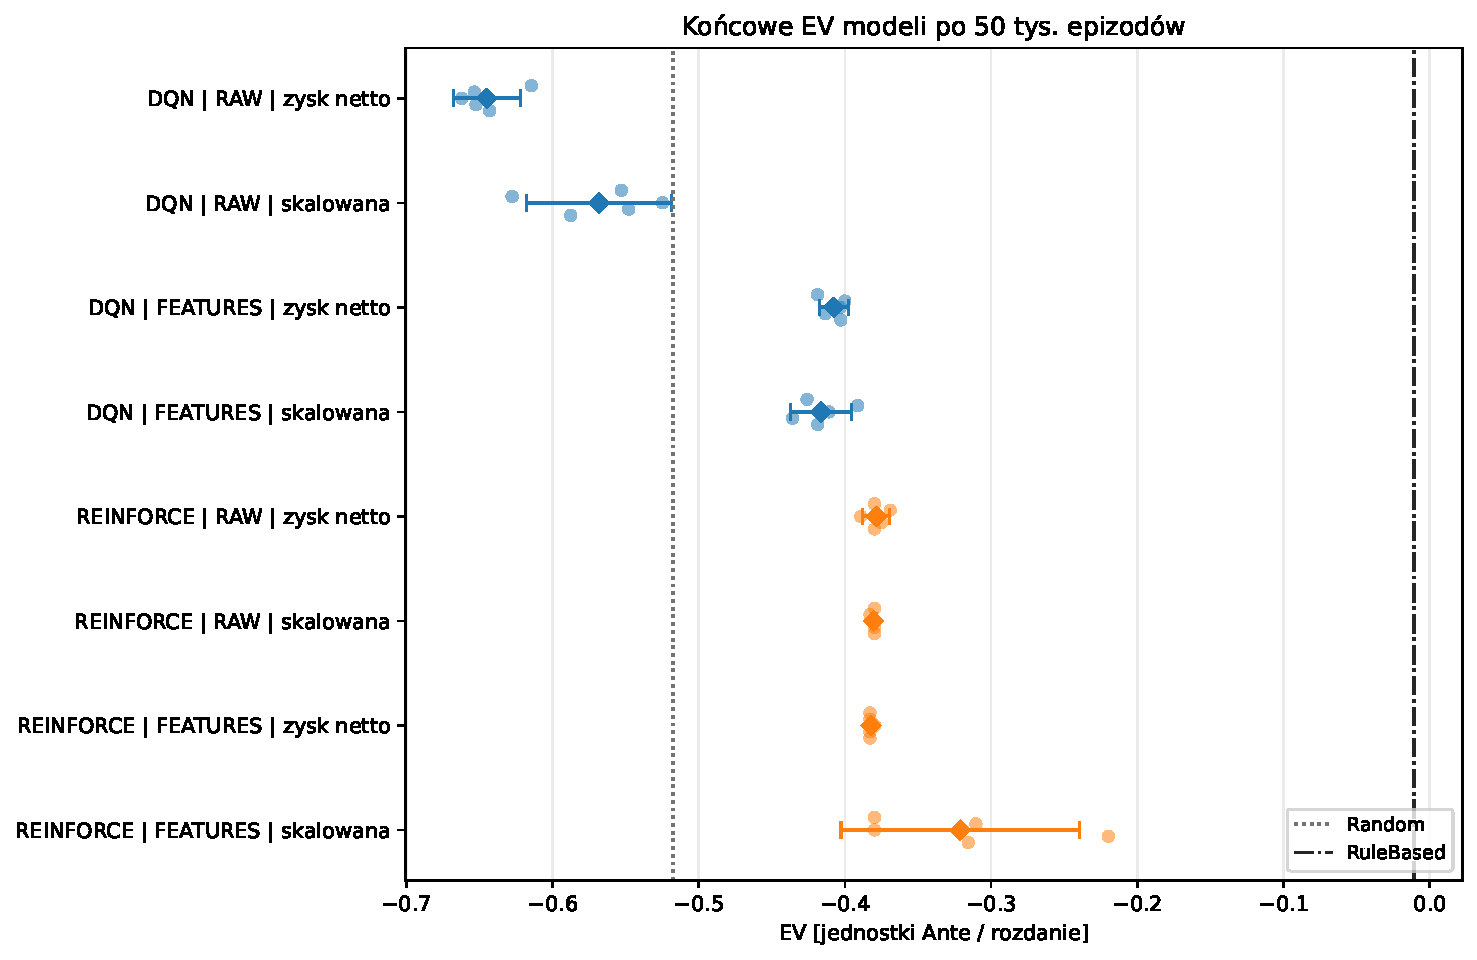
\includegraphics[
        width=\textwidth
    ]{../experiments/results/final_analysis/01_final_ev_50k.pdf}
    \caption{Końcowe wartości EV ośmiu konfiguracji po 50\,000
    epizodów treningowych. Małe punkty przedstawiają wyniki
    poszczególnych seedów, a większe znaczniki średnie wartości
    konfiguracji wraz z 95-procentowymi przedziałami ufności
    wyznaczonymi na podstawie pięciu przebiegów treningowych.
    Linie pionowe oznaczają wyniki agentów Random i RuleBased.}
    \label{fig:final-ev-50k}
\end{figure}

Wyniki pokazują również, że sama informacja o zastosowanym algorytmie
nie wystarcza do oceny jakości uzyskanej strategii. Szczególnie
w przypadku DQN rezultat zmienia się silnie wraz ze sposobem
reprezentacji stanu. W przypadku REINFORCE największą różnicę pomiędzy
wariantami obserwuję dla połączenia reprezentacji FEATURES ze
skalowaną funkcją nagrody. W kolejnych sekcjach analizuję oba czynniki
oddzielnie, wykorzystując sparowanie tych samych seedów treningowych.

\section{Wpływ reprezentacji stanu}
\label{sec:wyniki-reprezentacja-stanu}

W celu oceny wpływu sposobu reprezentacji stanu porównałem warianty
RAW i FEATURES przy zachowaniu tego samego algorytmu, funkcji nagrody
oraz seedu treningowego. Dla każdej pary wyznaczyłem różnicę

\begin{equation}
    \Delta EV_{\mathrm{state}}
    =
    EV_{\mathrm{FEATURES}}
    -
    EV_{\mathrm{RAW}}.
\end{equation}

Dodatnia wartość różnicy oznacza zatem przewagę reprezentacji
FEATURES. Porównanie wykonałem osobno dla obu algorytmów i obu funkcji
nagrody. Jednostką porównania jest w tym przypadku seed treningowy,
dlatego każda wartość średnia oraz odpowiadający jej przedział ufności
wynikają z pięciu sparowanych różnic.

W przypadku DQN zastosowanie reprezentacji FEATURES doprowadziło do
wyraźnej poprawy końcowego EV dla obu funkcji nagrody. Przy nagrodzie
opartej bezpośrednio na zysku netto średnia różnica wyniosła

\begin{equation}
    \Delta EV_{\mathrm{state}}
    =
    0{,}2374,
\end{equation}

a 95-procentowy przedział ufności był równy

\begin{equation}
    [0{,}2066,\ 0{,}2682].
\end{equation}

Dla skalowanej funkcji nagrody średnia różnica wyniosła
$0{,}1517$, przy 95-procentowym przedziale ufności
$[0{,}0863,\ 0{,}2170]$.

W obu przypadkach cały przedział znajduje się powyżej zera.
Wyniki wskazują więc, że w badanej konfiguracji DQN rozszerzenie
wektora stanu o cechy opisujące sytuację pokerową poprawiało jakość
uzyskiwanej strategii w sposób powtarzalny pomiędzy pięcioma
przebiegami treningowymi.

Dla REINFORCE wpływ reprezentacji stanu był znacznie mniej
jednoznaczny. Przy funkcji nagrody opartej na zysku netto średnia
różnica FEATURES względem RAW wyniosła $-0{,}0037$, a jej
95-procentowy przedział ufności
$[-0{,}0144,\ 0{,}0069]$ obejmował zero. Oznacza to, że w tym
wariancie obie reprezentacje prowadziły do bardzo podobnych wyników
końcowych.

Przy skalowanej funkcji nagrody średnia różnica wyniosła
$0{,}0593$, jednak przedział ufności był znacznie szerszy
i wyniósł $[-0{,}0225,\ 0{,}1411]$. Punktowe oszacowanie wskazuje
na wyższe EV reprezentacji FEATURES, ale duże zróżnicowanie wyników
między seedami nie pozwala uznać tego efektu za równie stabilny jak
w przypadku DQN.

Zestawienie wszystkich czterech porównań przedstawiam na
rysunku~\ref{fig:state-representation-effect}.

\begin{figure}[htbp]
    \centering
    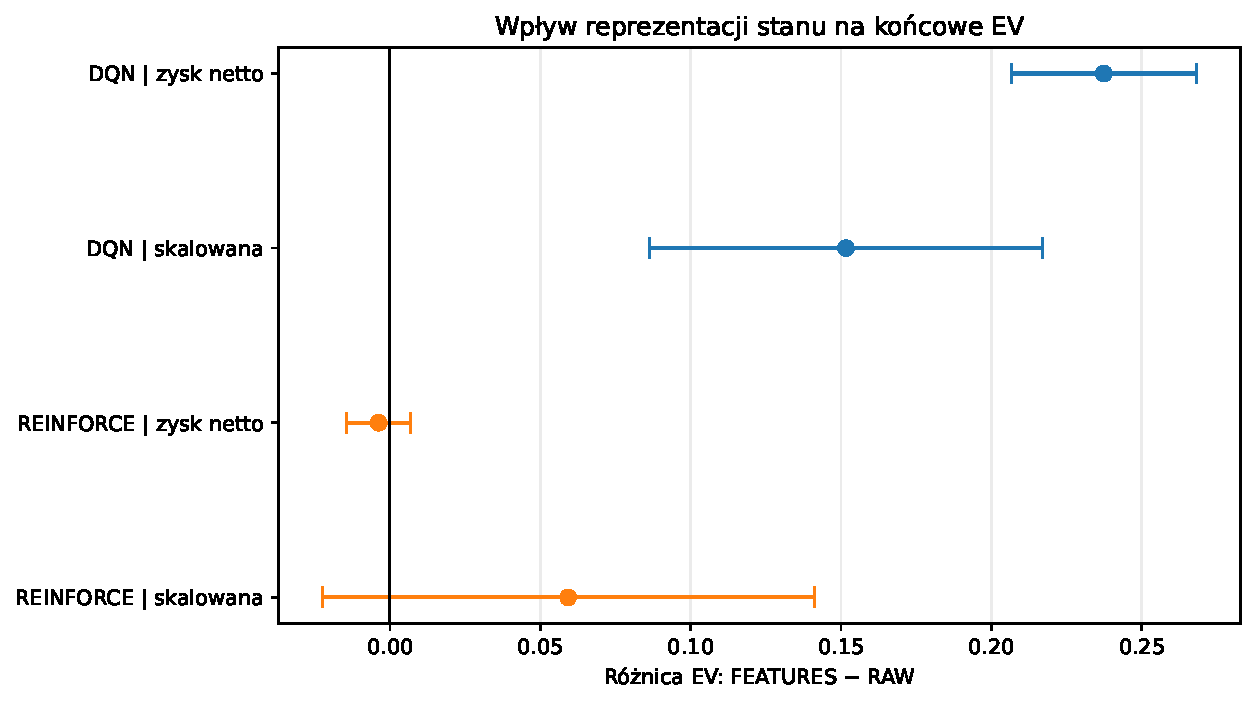
\includegraphics[
        width=0.9\textwidth
    ]{../experiments/results/final_analysis/02_state_representation_effect.pdf}
    \caption{Wpływ reprezentacji stanu na końcowe EV. Punkty
    przedstawiają średnią różnicę $EV_{\mathrm{FEATURES}} -
    EV_{\mathrm{RAW}}$ dla pięciu sparowanych seedów treningowych,
    a wąsy odpowiadają 95-procentowym przedziałom ufności.
    Wartości dodatnie oznaczają przewagę reprezentacji FEATURES.}
    \label{fig:state-representation-effect}
\end{figure}

Rezultaty wskazują zatem na wyraźnie odmienny wpływ reprezentacji
stanu na oba badane algorytmy. DQN korzystał wyraźnie z informacji zawartych
w rozszerzonej reprezentacji FEATURES, natomiast dla REINFORCE
nie zaobserwowałem równie stabilnego efektu zmiany reprezentacji.


\section{Wpływ funkcji nagrody}
\label{sec:wyniki-funkcja-nagrody}

Drugim badanym elementem była funkcja nagrody. Porównałem bezpośredni
zysk netto z jego wersją przeskalowaną przy zachowaniu tego samego
algorytmu, reprezentacji stanu oraz seedu treningowego. Różnicę
zdefiniowałem jako

\begin{equation}
    \Delta EV_{\mathrm{reward}}
    =
    EV_{\mathrm{net}}
    -
    EV_{\mathrm{scaled}}.
\end{equation}

Wartość dodatnia oznacza zatem przewagę bezpośredniego zysku netto,
natomiast ujemna przewagę nagrody skalowanej.

Dla DQN wykorzystującego reprezentację RAW średnia różnica wyniosła
$-0{,}0769$, a jej 95-procentowy przedział ufności był równy
$[-0{,}1314,\ -0{,}0224]$. W tym wariancie skalowanie nagrody
prowadziło więc do lepszych wyników końcowych w porównaniu
z bezpośrednim wykorzystaniem zysku netto.

Sytuacja wyglądała inaczej po zastosowaniu reprezentacji FEATURES.
Średnia różnica wyniosła jedynie $0{,}0089$, przy przedziale
$[-0{,}0057,\ 0{,}0234]$. Różnica jest niewielka, a przedział
obejmuje zero, dlatego na podstawie tych wyników nie można wskazać
wyraźnej przewagi jednej z funkcji nagrody dla DQN korzystającego
z reprezentacji FEATURES.

Podobny brak jednoznacznej przewagi wystąpił dla REINFORCE z
reprezentacją RAW. Średnia różnica wyniosła $0{,}0018$, natomiast
95-procentowy przedział ufności
$[-0{,}0087,\ 0{,}0124]$ obejmował zero.

Największą różnicę punktową dla REINFORCE zaobserwowałem przy
reprezentacji FEATURES. W tym przypadku wartość
$EV_{\mathrm{net}} - EV_{\mathrm{scaled}}$ wyniosła
$-0{,}0612$, czyli wyższy średni wynik osiągnęła funkcja skalowana.
Jednocześnie przedział ufności był bardzo szeroki i wyniósł
$[-0{,}1437,\ 0{,}0213]$. Wynik ten jest zgodny z dużym
zróżnicowaniem końcowej jakości polityk REINFORCE obserwowanym
pomiędzy seedami.

Porównania przedstawiam na
rysunku~\ref{fig:reward-effect}.

\begin{figure}[htbp]
    \centering
    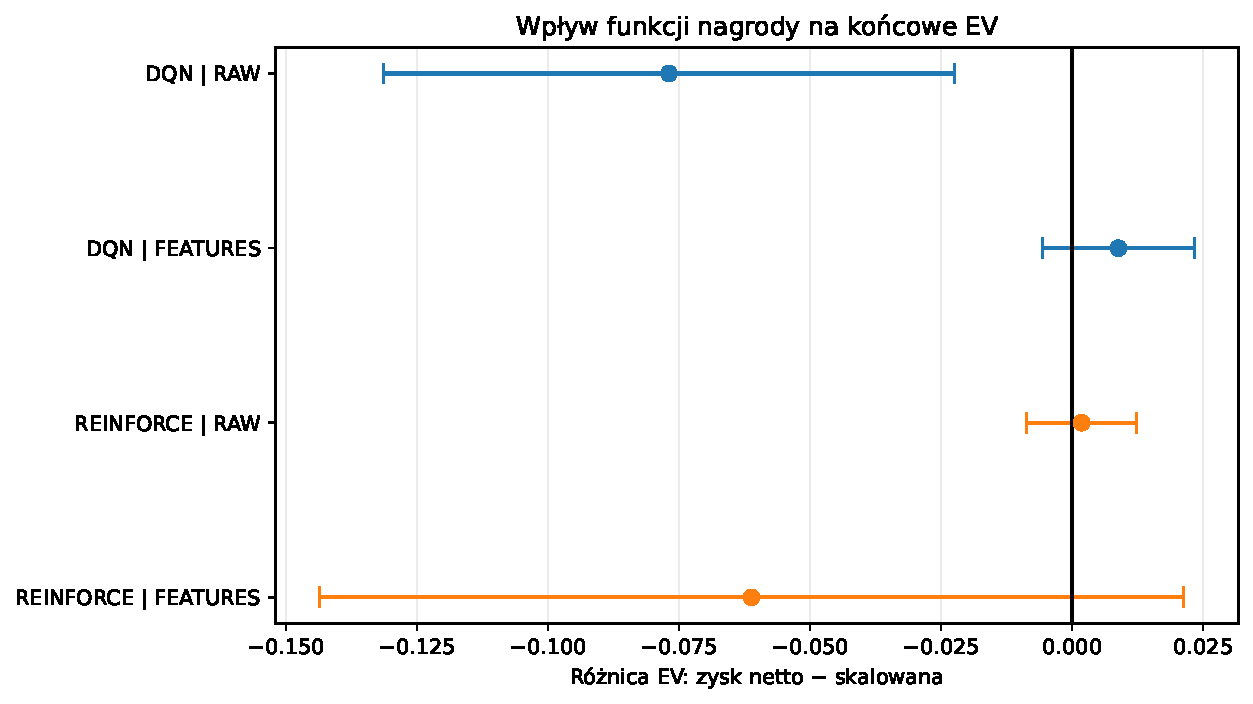
\includegraphics[
        width=0.9\textwidth
    ]{../experiments/results/final_analysis/03_reward_effect.pdf}
    \caption{Wpływ funkcji nagrody na końcowe EV. Punkty
    przedstawiają średnią różnicę $EV_{\mathrm{net}} -
    EV_{\mathrm{scaled}}$ dla pięciu sparowanych seedów
    treningowych, a wąsy odpowiadają 95-procentowym przedziałom
    ufności.}
    \label{fig:reward-effect}
\end{figure}

W przeciwieństwie do reprezentacji stanu nie obserwuję więc
uniwersalnego efektu skalowania funkcji nagrody. Jego wpływ zależy od
połączenia z algorytmem oraz sposobem reprezentacji stanu. Skalowanie
poprawiło wyniki DQN korzystającego z reprezentacji RAW, lecz dla DQN
z reprezentacją FEATURES różnica była niewielka. W przypadku
REINFORCE punktowo najlepszy wynik uzyskała konfiguracja FEATURES ze
skalowaną nagrodą, ale wynik ten był jednocześnie silnie zależny od
seedu treningowego.

\section{Przebieg procesu uczenia}
\label{sec:wyniki-przebieg-uczenia}

Końcowa ewaluacja pozwala porównać jakość wytrenowanych polityk,
ale nie pokazuje, w jaki sposób wynik ten kształtował się podczas
treningu. W tym celu wykorzystuję okresowe pomiary walidacyjne
wykonywane zgodnie z procedurą opisaną w
rozdziale~\ref{chap:eksperymenty}. Każdy punkt krzywej odpowiada
ewaluacji aktualnej polityki na 2\,000 wspólnych rozdań
walidacyjnych.

Wyniki walidacyjne traktuję jako opis dynamiki procesu uczenia,
a nie jako zamiennik końcowej ewaluacji na 100\,000 niezależnych
rozdań. Mniejsza liczba rozdań w pojedynczym punkcie powoduje większą
zmienność oszacowanego EV, jednak wspólny harmonogram walidacyjny
umożliwia bezpośrednie porównywanie kolejnych checkpointów.

Na rysunku~\ref{fig:dqn-learning-curves} przedstawiam przebieg
treningu czterech konfiguracji DQN.

\begin{figure}[htbp]
    \centering
    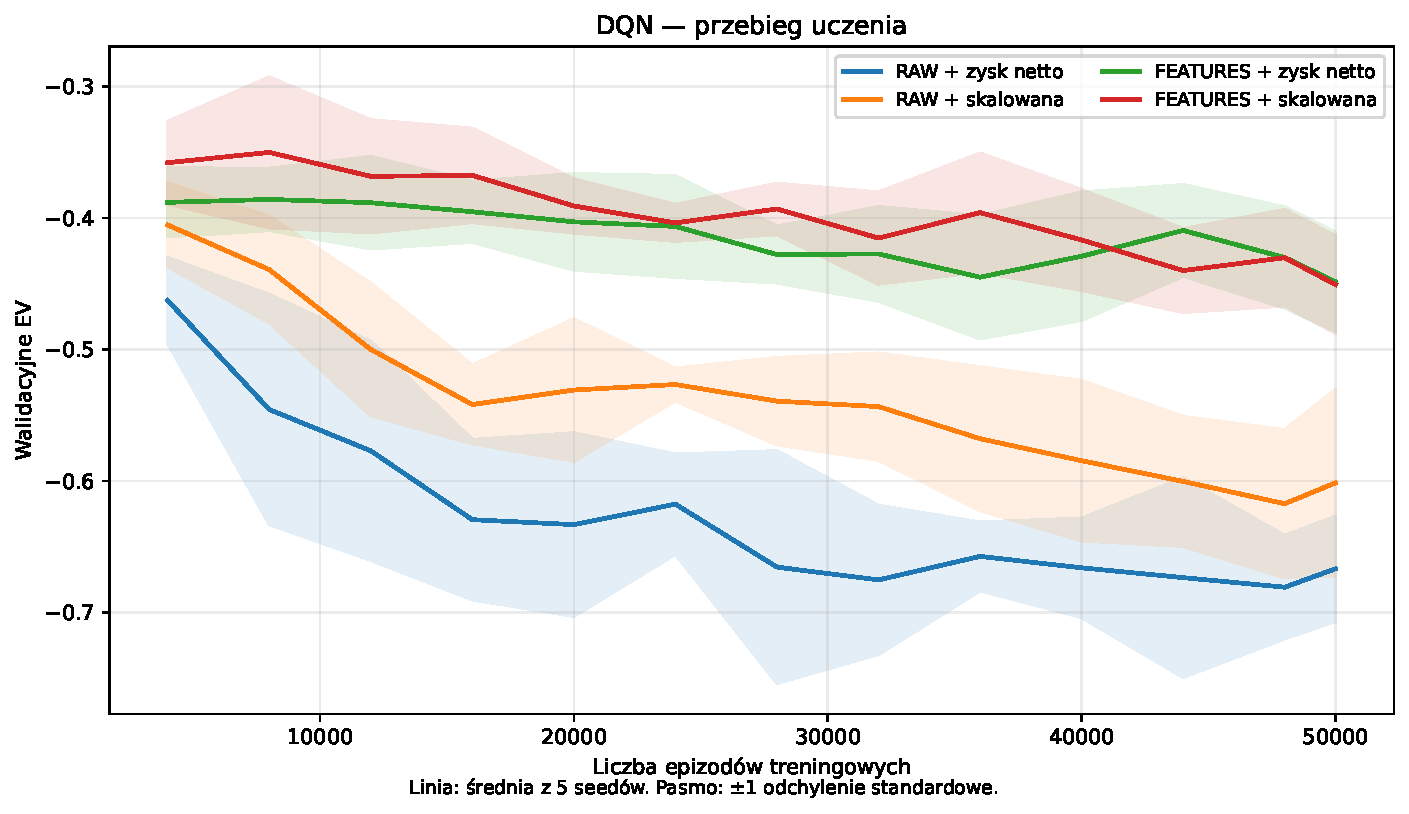
\includegraphics[
        width=\textwidth
    ]{../experiments/results/final_analysis/04_dqn_learning_curves.pdf}
    \caption{Przebieg uczenia czterech konfiguracji DQN.
    Linie przedstawiają średnie walidacyjne EV z pięciu seedów,
    natomiast pasma odpowiadają jednemu odchyleniu standardowemu
    między przebiegami treningowymi.}
    \label{fig:dqn-learning-curves}
\end{figure}

Już w trakcie treningu widoczna jest różnica pomiędzy
reprezentacjami RAW i FEATURES. Oba warianty wykorzystujące FEATURES
utrzymują przeciętnie wyższe EV niż odpowiadające im warianty RAW.
Jest to zgodne z wynikami końcowej ewaluacji przedstawionymi
w sekcji~\ref{sec:wyniki-reprezentacja-stanu}.

Jednocześnie krzywe nie wykazują monotonicznego wzrostu jakości
polityki. Po okresach poprawy występują lokalne spadki wartości
walidacyjnego EV. Oznacza to, że dalsze wykonywanie aktualizacji sieci
nie gwarantuje poprawy strategii na każdym kolejnym checkpointcie.
Zjawisko to występuje również dla konfiguracji FEATURES, które
ostatecznie uzyskały najwyższe wyniki spośród wariantów DQN.

Analogiczne wyniki dla REINFORCE przedstawiam na
rysunku~\ref{fig:reinforce-learning-curves}.

\begin{figure}[htbp]
    \centering
    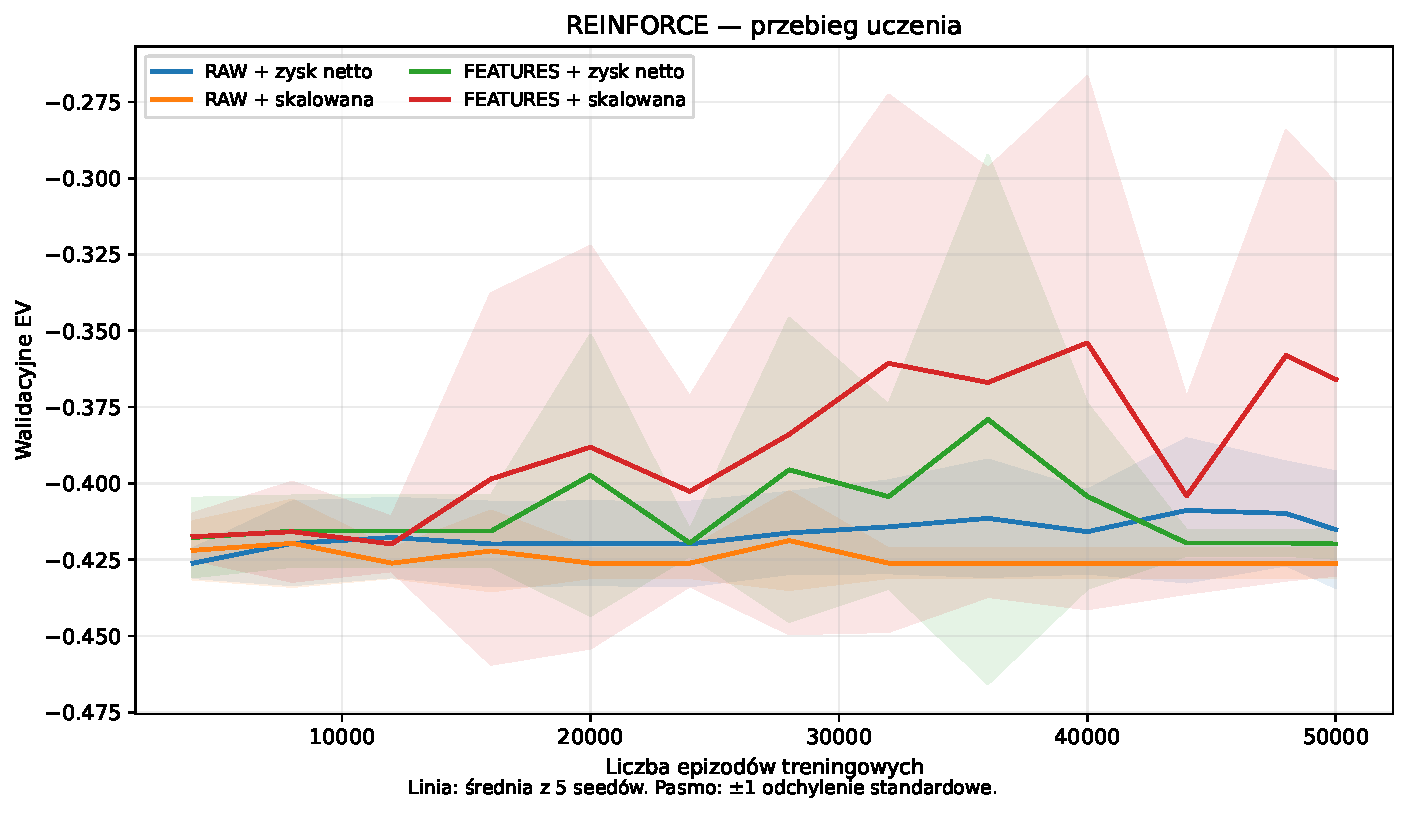
\includegraphics[
        width=\textwidth
    ]{../experiments/results/final_analysis/05_reinforce_learning_curves.pdf}
    \caption{Przebieg uczenia czterech konfiguracji REINFORCE.
    Linie przedstawiają średnie walidacyjne EV z pięciu seedów,
    a pasma jedno odchylenie standardowe między przebiegami
    treningowymi.}
    \label{fig:reinforce-learning-curves}
\end{figure}

W przypadku REINFORCE zależności pomiędzy konfiguracjami są mniej
regularne niż dla DQN. Szczególnie widoczne są okresy zwiększonego
rozrzutu pomiędzy seedami, podczas których poszczególne przebiegi tej
samej konfiguracji prowadzą do polityk o wyraźnie różnej jakości.

Najbardziej widoczne jest to dla konfiguracji FEATURES ze skalowaną
funkcją nagrody. Wariant ten osiągnął najwyższe średnie EV spośród
konfiguracji REINFORCE w końcowej ewaluacji, ale jednocześnie
charakteryzował się największym odchyleniem standardowym między
seedami. Krzywe walidacyjne pokazują, że zróżnicowanie to powstaje już
podczas procesu uczenia i nie jest wyłącznie efektem końcowej
ewaluacji.


\section{Wpływ zwiększenia budżetu treningowego}
\label{sec:wyniki-budzet-treningowy}

Po zakończeniu podstawowych eksperymentów rozszerzyłem trening dwóch
konfiguracji wybranych na podstawie wyników walidacyjnych. Dla DQN
była to konfiguracja FEATURES z nagrodą opartą na zysku netto,
natomiast dla REINFORCE konfiguracja FEATURES ze skalowaną funkcją
nagrody. Wszystkie pięć seedów obu konfiguracji kontynuowałem do
100\,000 epizodów.

Trajektorie poszczególnych seedów przedstawiam na
rysunku~\ref{fig:extended-training-per-seed}.

\begin{figure}[htbp]
    \centering
    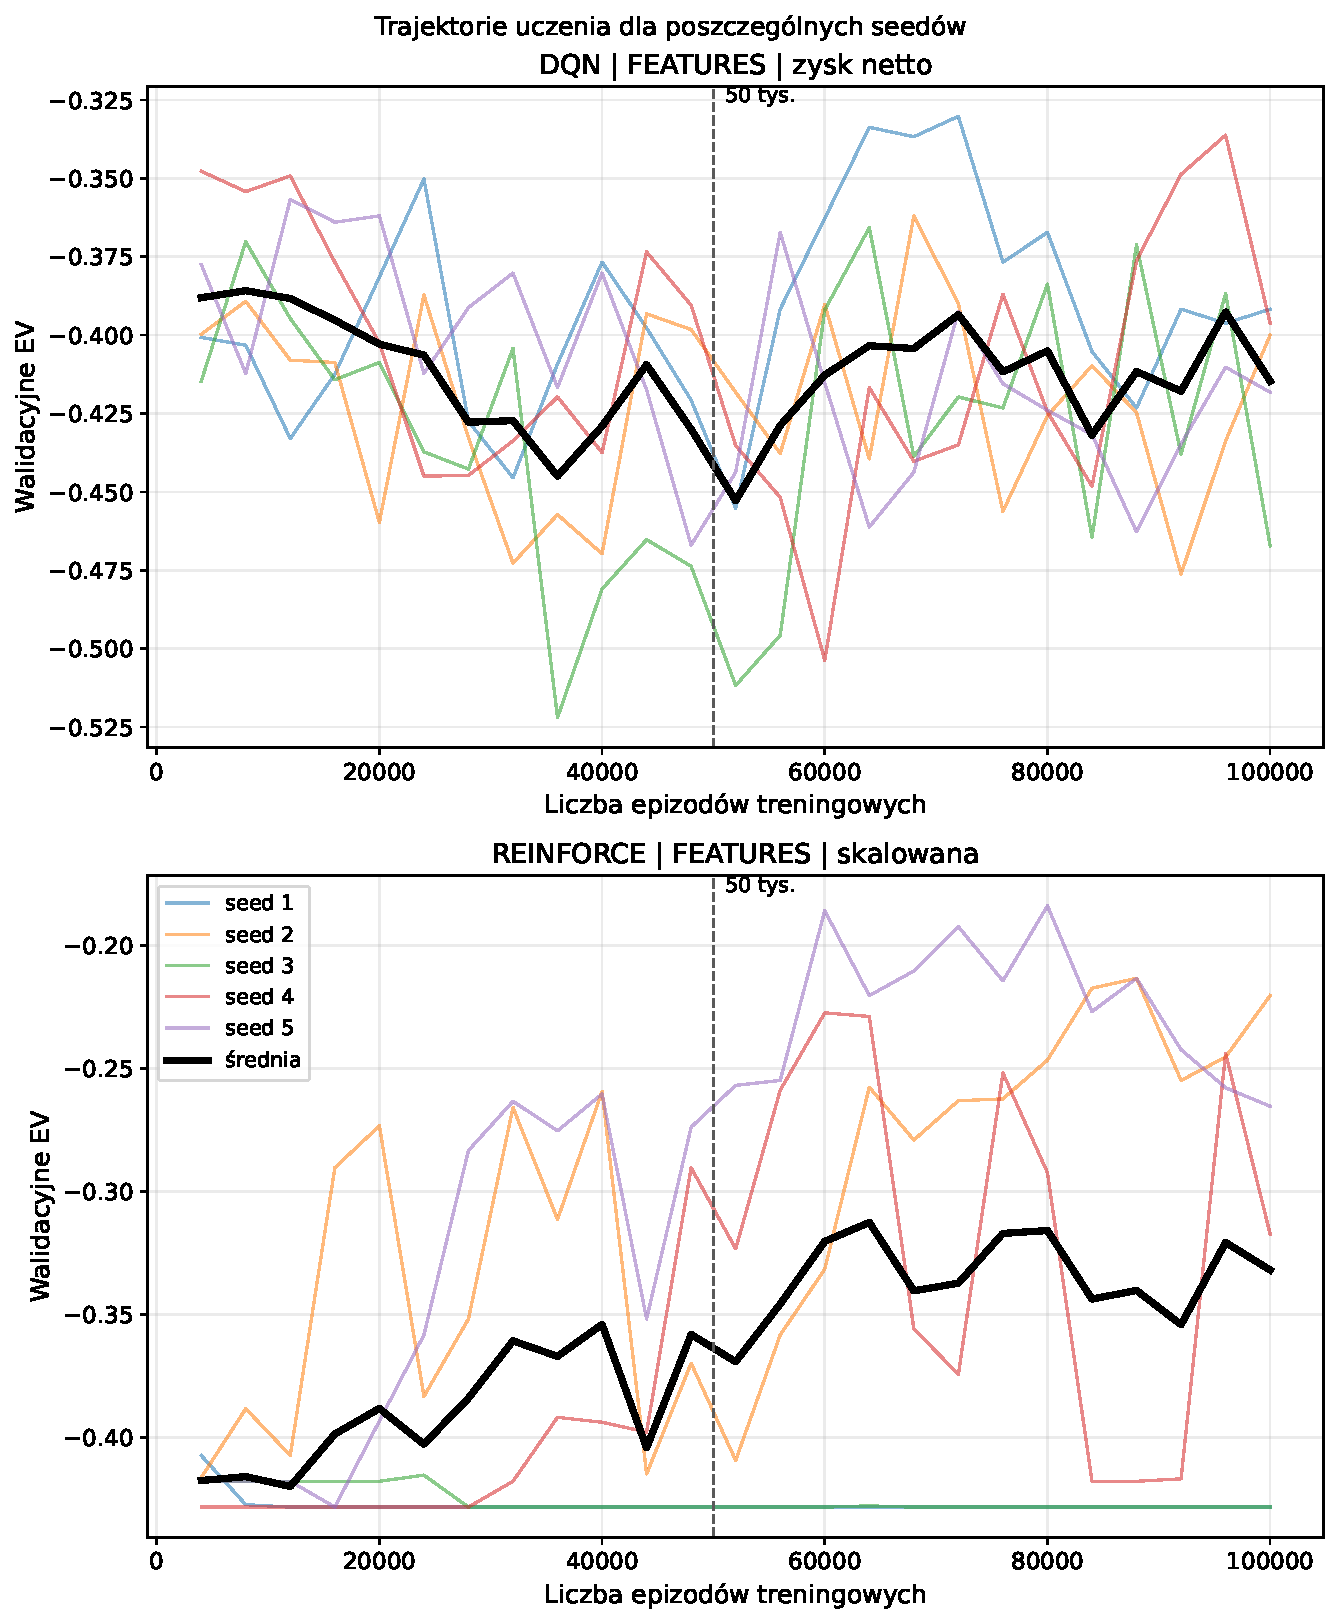
\includegraphics[
        width=\textwidth
    ]{../experiments/results/final_analysis/10_extended_training_per_seed.pdf}
    \caption{Trajektorie walidacyjnego EV dla pięciu seedów
    wybranych konfiguracji DQN i REINFORCE podczas treningu do
    100\,000 epizodów. Linia pionowa oznacza podstawowy budżet
    50\,000 epizodów.}
    \label{fig:extended-training-per-seed}
\end{figure}

Dla DQN wydłużenie treningu prowadziło do stosunkowo spójnej poprawy.
W końcowej ewaluacji na wspólnych 100\,000 rozdaniach średnie EV
pięciu modeli wzrosło z $-0{,}4076$ po 50\,000 epizodów do
$-0{,}3859$ po 100\,000 epizodów. Średnia sparowana poprawa wyniosła

\begin{equation}
    \Delta EV_{\mathrm{100k-50k}}
    =
    0{,}0217,
\end{equation}

a 95-procentowy przedział ufności po pięciu seedach był równy
$[0{,}0022,\ 0{,}0412]$.

Co istotne, poprawę końcowego EV zaobserwowałem dla wszystkich pięciu
seedów DQN. Nie oznacza to monotonicznej poprawy na każdym etapie
treningu, co widać na krzywych walidacyjnych, ale rezultat po
100\,000 epizodów był dla każdego seedu lepszy niż wynik odpowiadającego
mu modelu po 50\,000 epizodów.

Dla REINFORCE średnie EV wzrosło z $-0{,}3211$ do $-0{,}2943$.
Średnia różnica wyniosła $0{,}0268$, a więc punktowo była nawet
większa niż dla DQN. Jej 95-procentowy przedział ufności był jednak
równy $[-0{,}0362,\ 0{,}0898]$ i obejmował zero.

Wynik ten był konsekwencją dużego zróżnicowania zmian pomiędzy
poszczególnymi seedami. Niektóre przebiegi REINFORCE poprawiły się
znacznie, podczas gdy inne praktycznie nie zmieniły zachowania lub
uzyskały nieznacznie gorszy wynik. Wydłużenie treningu poprawiło więc
średni rezultat tej konfiguracji, ale nie usunęło problemu
niestabilności procesu uczenia.

Wyniki rozszerzenia budżetu podsumowuję w
tabeli~\ref{tab:extended-training-results}.

\begin{table}[htbp]
    \centering
    \caption{Wpływ zwiększenia budżetu treningowego z 50\,000 do
    100\,000 epizodów}
    \label{tab:extended-training-results}
    \begin{tabular}{lrrrr}
        \toprule
        Algorytm & EV 50k & EV 100k & Różnica & 95\% CI \\
        \midrule
        DQN
            & -0{,}4076
            & -0{,}3859
            & 0{,}0217
            & [0{,}0022,\ 0{,}0412] \\
        REINFORCE
            & -0{,}3211
            & -0{,}2943
            & 0{,}0268
            & [-0{,}0362,\ 0{,}0898] \\
        \bottomrule
    \end{tabular}
\end{table}

Rozszerzony eksperyment należy traktować jako analizę uzupełniającą.
Podstawowe porównania reprezentacji stanu i funkcji nagrody pozostają
oparte na pełnej macierzy eksperymentalnej przy wspólnym budżecie
50\,000 epizodów.


\section{Stabilność procesu uczenia}
\label{sec:wyniki-stabilnosc}

Różnice między DQN i REINFORCE są widoczne nie tylko w średnim EV,
ale również w powtarzalności procesu treningowego. W celu
przedstawienia tego zjawiska obliczyłem dla kolejnych checkpointów
odchylenie standardowe walidacyjnego EV pomiędzy pięcioma seedami
wybranych konfiguracji.

Wyniki przedstawiam na
rysunku~\ref{fig:seed-variability-over-training}.

\begin{figure}[htbp]
    \centering
    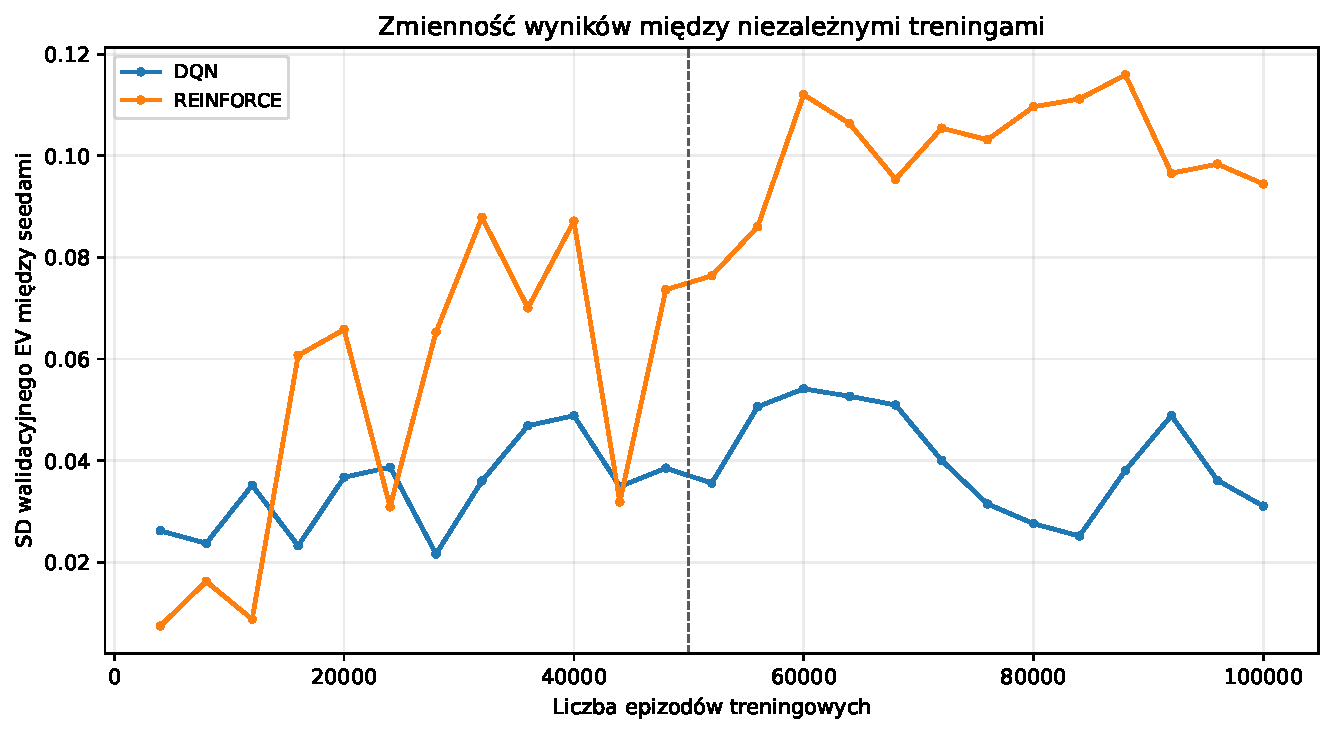
\includegraphics[
        width=0.9\textwidth
    ]{../experiments/results/final_analysis/08_seed_variability_over_training.pdf}
    \caption{Zmienność walidacyjnego EV pomiędzy pięcioma seedami
    podczas treningu wybranych konfiguracji DQN i REINFORCE.
    Oś pionowa przedstawia odchylenie standardowe wartości EV między
    przebiegami treningowymi.}
    \label{fig:seed-variability-over-training}
\end{figure}

DQN utrzymywał relatywnie niewielki rozrzut pomiędzy niezależnymi
przebiegami. REINFORCE wykazywał natomiast okresy znacznie większej
zmienności, co jest zgodne zarówno z krzywymi uczenia, jak i wynikami
końcowej ewaluacji. Oznacza to, że w badanym ustawieniu REINFORCE
częściej prowadził do jakościowo różnych polityk pomimo wykorzystania
tej samej konfiguracji hiperparametrów.

Dodatkową informację o przebiegu optymalizacji daje analiza normy
gradientu. Na rysunku~\ref{fig:gradient-norm-reward-scale}
porównuję jej przebieg dla obu wariantów funkcji nagrody.

\begin{figure}[htbp]
    \centering
    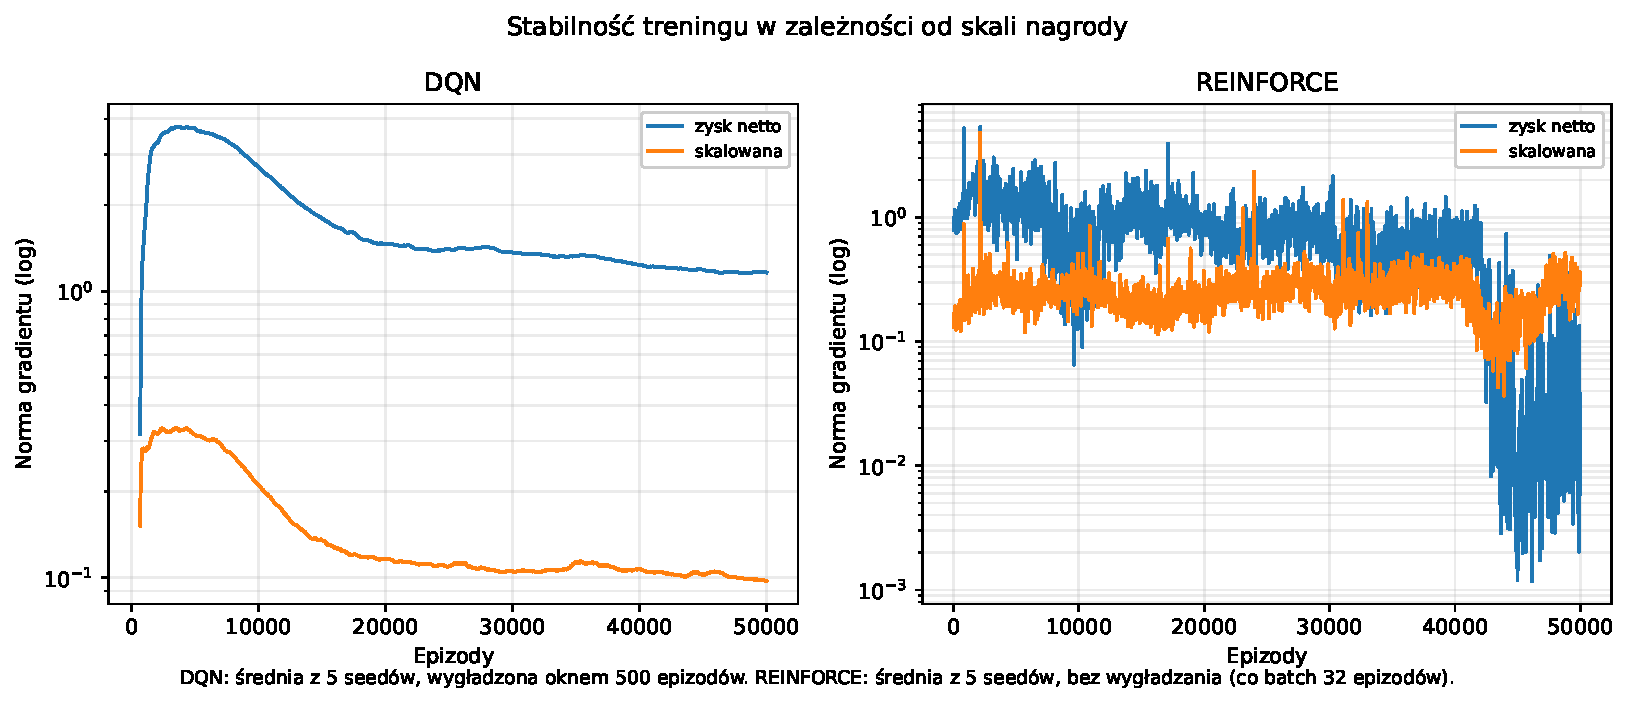
\includegraphics[
        width=\textwidth
    ]{../experiments/results/final_analysis/19_training_stability_by_reward_scale.pdf}
    \caption{Norma gradientu w zależności od skali funkcji nagrody
    dla konfiguracji wykorzystujących reprezentację FEATURES.
    Dla DQN przedstawiono średnią z pięciu seedów wygładzoną oknem
    500 epizodów, natomiast dla REINFORCE średnią z pięciu seedów
    bez dodatkowego wygładzania. Oś pionowa ma skalę logarytmiczną.}
    \label{fig:gradient-norm-reward-scale}
\end{figure}

Skalowanie nagrody wyraźnie zmieniało skalę gradientów powstających
podczas optymalizacji. Nie oznacza to jednak automatycznie poprawy
końcowej jakości polityki. Jak pokazały wyniki z
sekcji~\ref{sec:wyniki-funkcja-nagrody}, mniejsza skala sygnału
optymalizacyjnego nie przekładała się na uniwersalną przewagę
skalowanej funkcji nagrody.

Analiza gradientów stanowi zatem uzupełnienie wyników EV. Pokazuje,
że zmiana funkcji nagrody wpływa na przebieg aktualizacji parametrów,
ale sama kontrola skali gradientu nie rozwiązuje problemów związanych
ze stabilnością uczenia ani nie gwarantuje uzyskania lepszej
strategii.

\section{Analiza zachowania wyuczonych polityk}
\label{sec:wyniki-zachowanie-polityk}

Wartość EV opisuje końcową jakość strategii, ale nie pokazuje
bezpośrednio, jakie zachowanie zostało wyuczone przez agenta.
Z tego względu uzupełniłem analizę ilościową o analizę decyzji
podejmowanych przez wybrane konfiguracje DQN i REINFORCE.

Szczególnie interesujące zachowanie wystąpiło dla konfiguracji
REINFORCE FEATURES ze skalowaną funkcją nagrody. Jak pokazały
wcześniejsze wyniki, konfiguracja ta osiągała najwyższe średnie EV
spośród wariantów REINFORCE, ale charakteryzowała się również
największą zmiennością pomiędzy seedami.

Na rysunku~\ref{fig:reinforce-action-profiles} przedstawiam rozkład
akcji pięciu modeli tej konfiguracji po rozszerzeniu treningu do
100\,000 epizodów.

\begin{figure}[htbp]
    \centering
    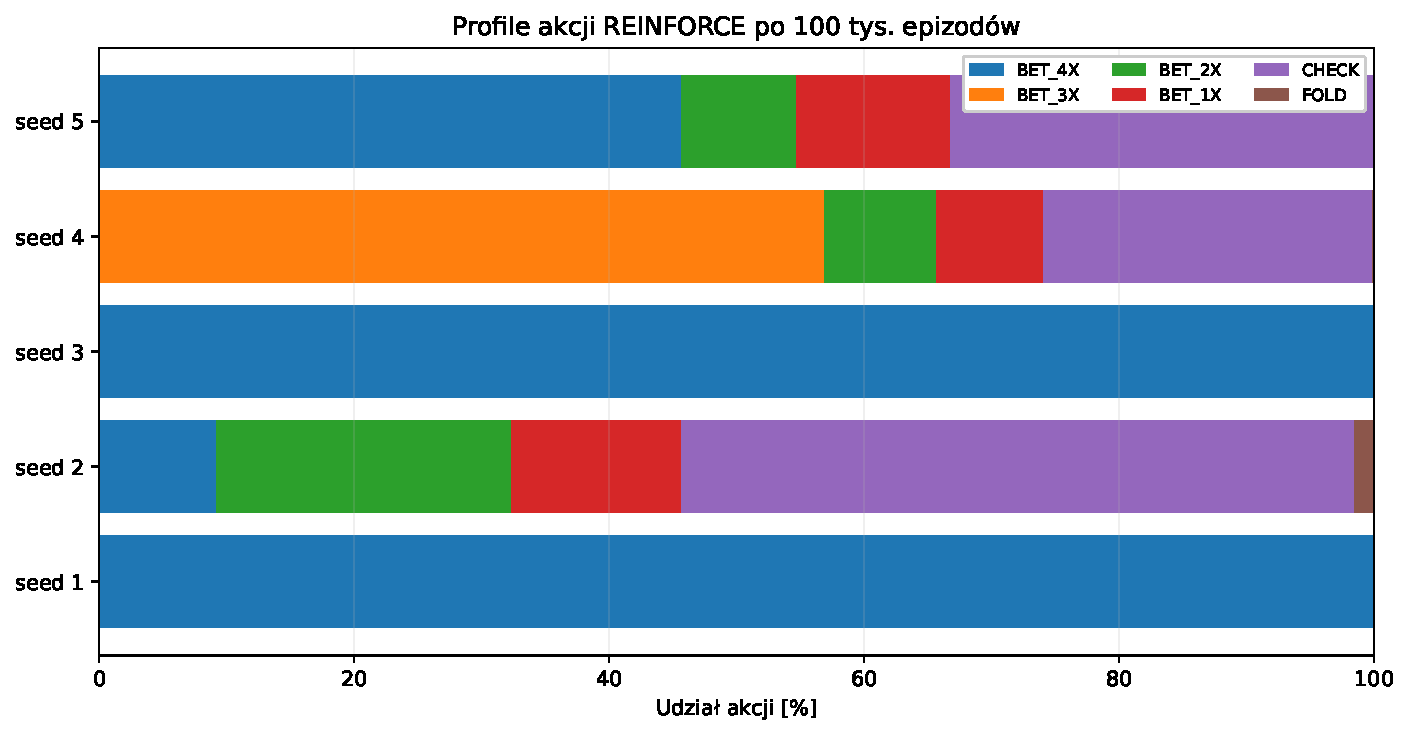
\includegraphics[
        width=\textwidth
    ]{../experiments/results/final_analysis/09_reinforce_action_profiles.pdf}
    \caption{Profile akcji pięciu modeli REINFORCE FEATURES ze
    skalowaną funkcją nagrody po 100\,000 epizodów treningowych.
    Każdy pasek przedstawia udział poszczególnych akcji w końcowej
    ewaluacji danego seedu.}
    \label{fig:reinforce-action-profiles}
\end{figure}

Profile poszczególnych seedów różnią się wyraźnie. Dwa z pięciu
modeli wybierały akcję \texttt{BET\_4X} we wszystkich 100\,000
rozdaniach końcowej ewaluacji. Oznacza to, że polityka tych modeli
uległa degeneracji do bardzo prostej strategii, w której decyzja
przed flopem przestała zależeć od obserwowanego stanu gry.

Pozostałe przebiegi prowadziły do bardziej zróżnicowanych polityk,
które podejmowały również decyzje zależne od kolejnych faz rozdania.
Wyjaśnia to część wysokiej zmienności wyników REINFORCE pomiędzy
seedami. Ta sama konfiguracja treningowa może prowadzić zarówno do
polityki wykorzystującej informacje ze stanu, jak i do rozwiązania
zdominowanego przez jedną akcję.

Co istotne, zwiększenie budżetu treningowego do 100\,000 epizodów nie
usunęło tego zjawiska. Dwa seedy pozostające w prostej polityce po
50\,000 epizodów nie zmieniły jej również podczas dalszego treningu.
Oznacza to, że sam wzrost liczby epizodów nie wystarczył do
wyprowadzenia tych przebiegów z osiągniętego rozwiązania.

Drugim sposobem analizy zachowania jest porównanie decyzji przed
flopem dla poszczególnych układów początkowych. Na
rysunku~\ref{fig:preflop-range-chart} przedstawiam dominujące decyzje
agenta regułowego oraz wybranych walidacyjnie konfiguracji DQN
i REINFORCE.

\begin{figure}[htbp]
    \centering
    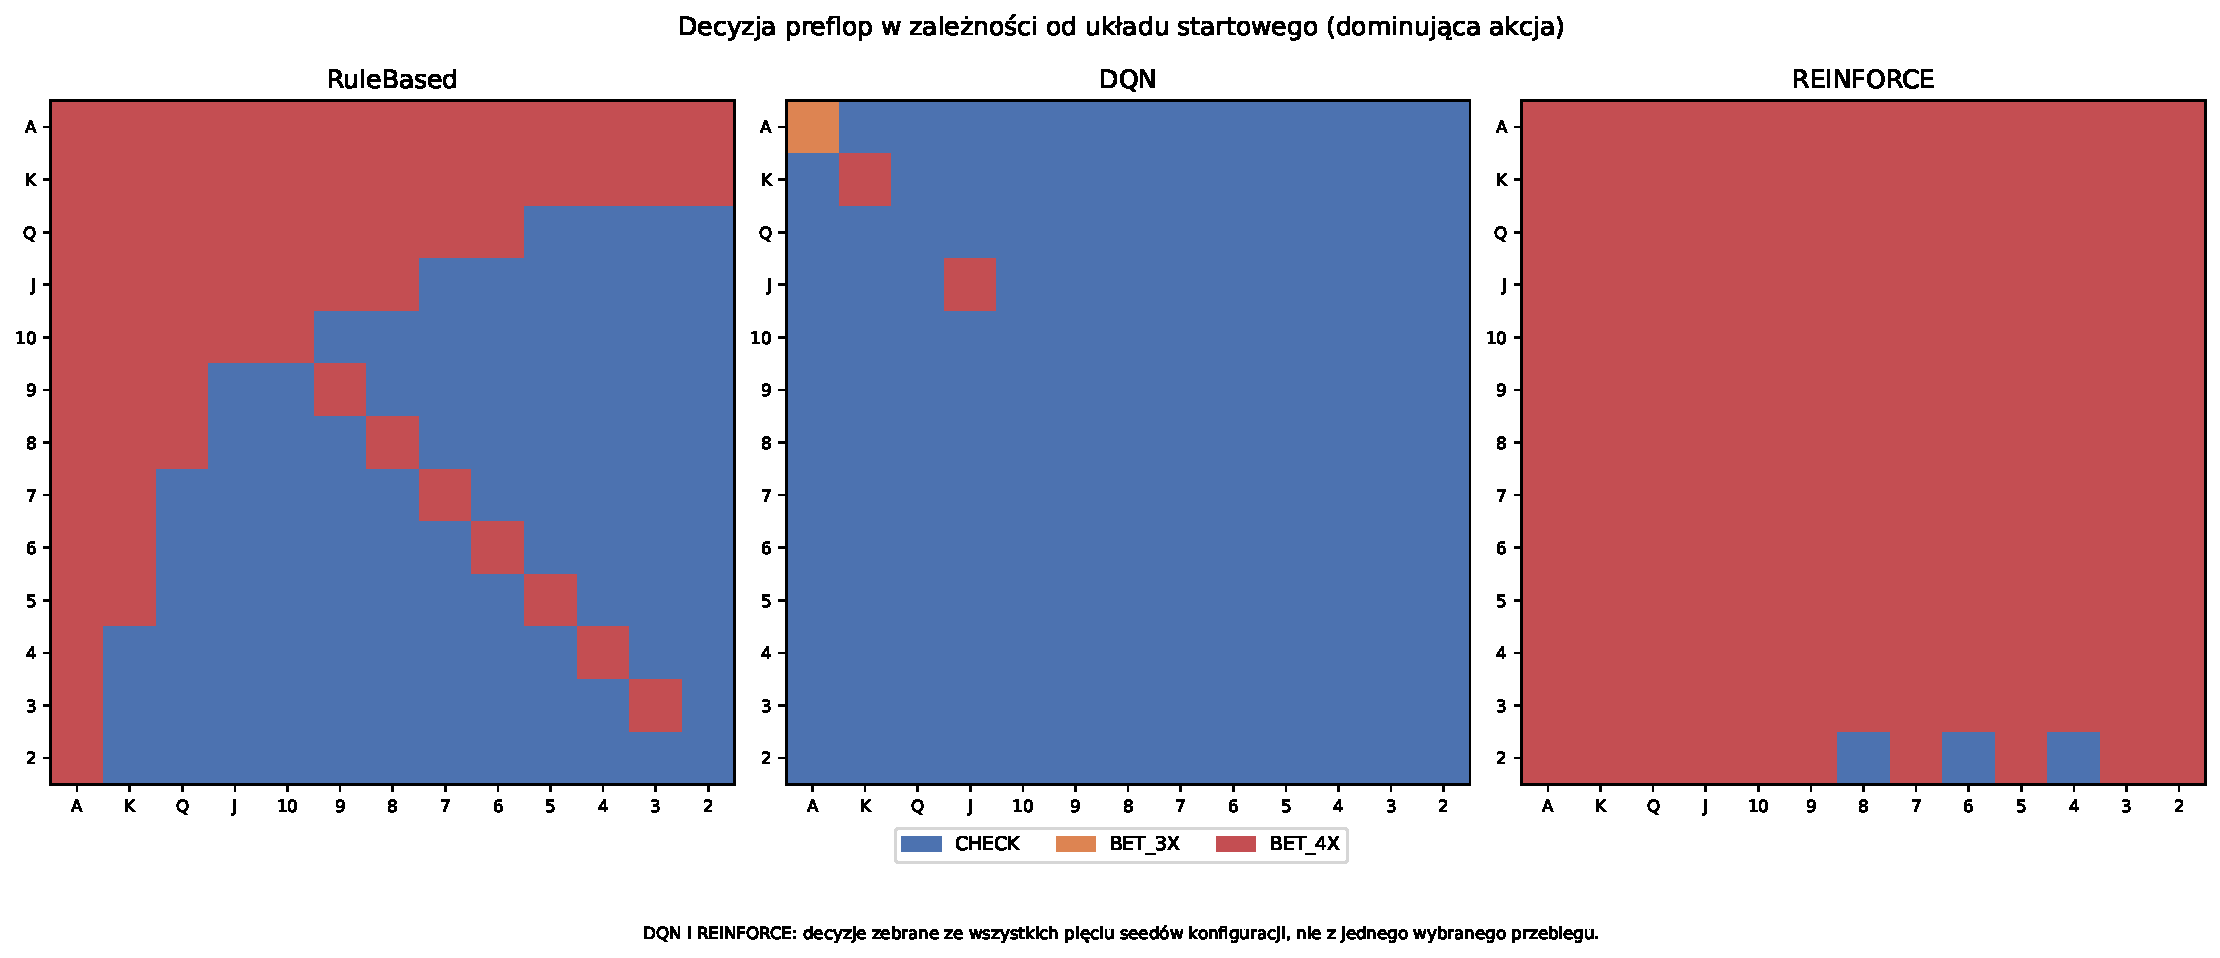
\includegraphics[
        width=\textwidth
    ]{../experiments/results/final_analysis/18_preflop_range_chart.pdf}
    \caption{Dominujące decyzje przed flopem w zależności od układu
    dwóch kart początkowych dla agenta RuleBased oraz wybranych
    walidacyjnie konfiguracji DQN i REINFORCE. Dla metod RL decyzje
    zagregowano po pięciu seedach treningowych.}
    \label{fig:preflop-range-chart}
\end{figure}

Agent regułowy posiada wyraźnie zdefiniowany obszar układów
początkowych, dla których wykonuje zakład \texttt{BET\_4X}, zgodny
z regułami strategii opisanymi w
rozdziale~\ref{sec:agent-regulowy}. Nauczone polityki tworzą inne
granice decyzyjne, wynikające wyłącznie z procesu optymalizacji
oczekiwanej nagrody.

Porównanie pokazuje, że modele RL nie odtworzyły wprost strategii
agenta regułowego. Jednocześnie ich zachowanie nie jest równoważne
strategii losowej. Szczególnie dla lepszych konfiguracji widoczne są
powtarzalne zależności pomiędzy układem początkowym i wybieraną akcją.
Oznacza to, że w trakcie treningu modele nauczyły się wykorzystywać
część informacji zawartej w obserwowanym stanie, mimo że końcowa
jakość strategii pozostawała niższa od jakości heurystyki RuleBased.


\section{Dyskusja wyników}
\label{sec:dyskusja-wynikow}

Przeprowadzone eksperymenty pokazują, że na jakość strategii
w Ultimate Texas Hold'em wpływa nie tylko wybór algorytmu uczenia,
ale również sposób przedstawienia stanu i właściwości procesu
optymalizacji.

Najbardziej jednoznaczny efekt zaobserwowałem dla reprezentacji stanu
w DQN. Rozszerzenie RAW o cechy pokerowe w reprezentacji FEATURES
poprawiło wynik dla obu funkcji nagrody i efekt ten wystąpił
konsekwentnie dla pięciu sparowanych seedów treningowych. Wynik ten
wskazuje, że w badanym budżecie treningowym jawne dostarczenie
informacji o strukturze sytuacji pokerowej ułatwia DQN wykorzystanie
dostępnej obserwacji.

Dla REINFORCE analogicznego, stabilnego efektu reprezentacji stanu
nie zaobserwowałem. Najwyższe średnie EV uzyskało połączenie FEATURES
ze skalowaną nagrodą, jednak było ono jednocześnie konfiguracją
o największej zmienności pomiędzy seedami. Wynik średni nie
odzwierciedla więc w tym przypadku typowego rezultatu pojedynczego
treningu równie dobrze jak dla DQN.

Wpływ skalowania nagrody również nie był uniwersalny. Dla DQN
korzystającego z reprezentacji RAW nagroda skalowana prowadziła do
wyższego EV, natomiast po zastosowaniu FEATURES różnica pomiędzy
funkcjami nagrody była niewielka. Diagnostyka norm gradientu
potwierdziła, że zmiana skali nagrody istotnie wpływa na wielkość
sygnału optymalizacyjnego, ale samo ograniczenie tej skali nie
gwarantuje poprawy końcowej polityki.

Porównując oba algorytmy przy podstawowym budżecie 50\,000 epizodów,
REINFORCE osiągnął wyższe średnie EV od DQN dla każdego
odpowiadającego sobie połączenia reprezentacji stanu i funkcji
nagrody. Nie oznacza to jednak jednoznacznej przewagi REINFORCE.
Wyniki tego algorytmu były bardziej zależne od seedu treningowego,
a część przebiegów prowadziła do degeneracji polityki do prostych
schematów decyzyjnych.

DQN osiągał niższe średnie EV, lecz proces treningowy był bardziej
powtarzalny. Również eksperyment z większym budżetem treningowym
wskazał na różnicę pomiędzy algorytmami. Wszystkie pięć modeli DQN
poprawiło wynik po zwiększeniu budżetu do 100\,000 epizodów,
natomiast dla REINFORCE poprawa była silnie zależna od konkretnego
seedu.

Żadna z badanych konfiguracji RL nie osiągnęła jakości strategii
RuleBased. Agent regułowy uzyskał w końcowej ewaluacji EV równe
$-0{,}0106$, podczas gdy najlepsze średnie wyniki podstawowych
konfiguracji RL pozostawały wyraźnie ujemne. Pokazuje to, że przy
zastosowanych architekturach, hiperparametrach i budżecie treningowym
prosta strategia wykorzystująca wiedzę dziedzinową pozostaje
znacznie skuteczniejsza.

Nie oznacza to jednak, że modele RL nie nauczyły się użytecznej
struktury problemu. Większość konfiguracji osiągnęła wynik wyższy od
agenta losowego, a analiza decyzji pokazała zależności pomiędzy
obserwowanym stanem i podejmowanymi akcjami. Wyniki sugerują więc,
że badane metody były zdolne do uczenia się strategii, lecz jakość
tej strategii pozostawała ograniczona.

Na interpretację wyników wpływają również ograniczenia przyjętego
zakresu eksperymentalnego. Dla obu algorytmów wykorzystałem jedną
ustaloną architekturę i jeden zestaw hiperparametrów. REINFORCE
pozostał metodą bez funkcji bazowej, krytyka i dodatkowej regularyzacji
entropii. Reprezentacja FEATURES zawiera natomiast ręcznie
zaprojektowane cechy pokerowe, dlatego jej przewaga nad RAW pokazuje
wartość tej konkretnej informacji dziedzinowej, a nie uniwersalną
przewagę każdej reprezentacji o większej liczbie cech.

Z tego względu wyników nie traktuję jako rozstrzygnięcia o ogólnej
wyższości jednego algorytmu nad drugim. Pokazują one natomiast
wyraźnie, że w badanym środowisku DQN i REINFORCE reagują inaczej na
reprezentację stanu, skalę nagrody i zwiększenie budżetu treningowego.
Różnica pomiędzy średnią jakością polityki a stabilnością jej
uzyskiwania stanowi jeden z najważniejszych rezultatów
przeprowadzonych eksperymentów.